%
% File naacl2019.tex
%
%% Based on the style files for ACL 2018 and NAACL 2018, which were
%% Based on the style files for ACL-2015, with some improvements
%%  taken from the NAACL-2016 style
%% Based on the style files for ACL-2014, which were, in turn,
%% based on ACL-2013, ACL-2012, ACL-2011, ACL-2010, ACL-IJCNLP-2009,
%% EACL-2009, IJCNLP-2008...
%% Based on the style files for EACL 2006 by 
%%e.agirre@ehu.es or Sergi.Balari@uab.es
%% and that of ACL 08 by Joakim Nivre and Noah Smith

\documentclass[11pt,a4paper]{article}
\usepackage[hyperref]{naaclhlt2019}
\usepackage{times}
\usepackage{latexsym}
\usepackage{graphicx}
\usepackage{enumerate}
\usepackage{multirow}
\usepackage{subcaption}

\usepackage{url}

\aclfinalcopy % Uncomment this line for the final submission
%\def\aclpaperid{***} %  Enter the acl Paper ID here

%\setlength\titlebox{5cm}
% You can expand the titlebox if you need extra space
% to show all the authors. Please do not make the titlebox
% smaller than 5cm (the original size); we will check this
% in the camera-ready version and ask you to change it back.

\newcommand\BibTeX{B{\sc ib}\TeX}

\title{How Good is a Chess Player?\\
    Prediction of Elo rankings based on Play-by-Play records}
\begin{document}
\maketitle
\section{Overview}
Chess has always been a fascinating combination of strategy and skill. Both during, and especially after a game, there are endless opportunities to analyze how the players went about their moves, what a board state at an instant in the game represented, which move turned the tables in favor of the winner and so on. The strength of chess players is translated into their respective Elo ratings, with players above a certain grade to be categorized as Grand Masters. Given that the performance of the players are mapped to Elo rankings, it should be possible to foretell the Elo rankings of a player by looking at the set of moves made by them in their games. Our main aim as part of this analysis is to create a model that predicts just that, the Elo rankings of the players involved in the game within a certain degree of confidence. Lichess is an online chess server that enables players to play online and analyze their games. All this data is available as part of a humongous repository which would form the essential dataset for this endeavor. 
Building up on our initial proposal and the mid-sem report, we employ extensive feature engineering to create novel attributes and quantify the corresponding moves of both a player and their opponent (White and Black). These features are then used for regression analysis by applying them to linear and random forest regression models and the results obtained are analyzed. As an additional exercise we applied the relative strength of the moves of each player to a deep learning model to classify their rankings as part of a particular range of players as well as try to predict the type of game a player was involved in.
The rest of the report is divided into the following sections:
\begin{itemize}
    \item Background
    \item Dataset
    \item Exploratory Data Analysis and Pre-processing
    \item Feature Engineering
    \item Methods
    \item Extended Work
    \item Results
    \item Conclusion
\end{itemize}
\section{Background}
Elo scores were initially created as a means to rank chess players. Since then, they have been
introduced in a lot of other fields and games like baseball, basketball and even video games. The primary concept is the zero-sum nature of the Elo score where the ratings between two players
serve as a predictor of the outcome of a match. The difference between the ratings of the winner and loser determines the total number of points gained or lost after a game.[5] 
\\Coming back to the roots of Elo ratings with Chess, the players at every level, students and analysts of the game keep a record of the moves played in the games they were a part of. The moves are represented in a standard format called the 'Algebraic Chess Notation' and generally chess enthusiasts maintain such a record in a scoring sheet. Thankfully, with the advent and popularity of online chess tournaments, many online portals have come to the fore which have huge repositories of game data in Portable Game Notation files \cite{PGN} and these form the basis of our analysis. Lichess.org\cite{Lichess} is one such portal,  that enables players to both play online and analyze their games through the embedded Stockfish Chess Engine\cite{Stockfish}. Given that the PGN data has all the moves, Elo Rankings of both the involved players and other metadata, this becomes the perfect recipe for a machine learning problem where in given the moves and metadata of a set of games, we employ a model to predict the Elo Rankings of the players involved. This seems logical as higher the ranking of a player, the better his/her skills are and more informed their choice of moves would be.


\section{Dataset}
As mentioned previously, we used a PGN files from Lichess which has game data of 100,000 games. The particular dataset used for this project is from February 2013. One of the challenges was to get this data in a readable format that could be used for data analysis. We created a Python based pipeline to generate a CSV file for the game data which can then be directly loaded as a Pandas DataFrame. We added extra steps to gather additional information from the moves itself during this conversion of PGN to CSV. This was done to ease our work on the bits which might not be straight forward once we moved to the CSV format. eg. Some  of the critical pieces of information we captured was the number of pieces attacking the 4 center squares (E4, E4, D4 and D5) for both Black and White at any giving instant as we traverse the moves in the PGN file. This was relatively easy thanks to the python-chess API\cite{pythonchess} and would not have been straightforward later during feature engineering.
\begin{figure}[!ht]
    \centering
    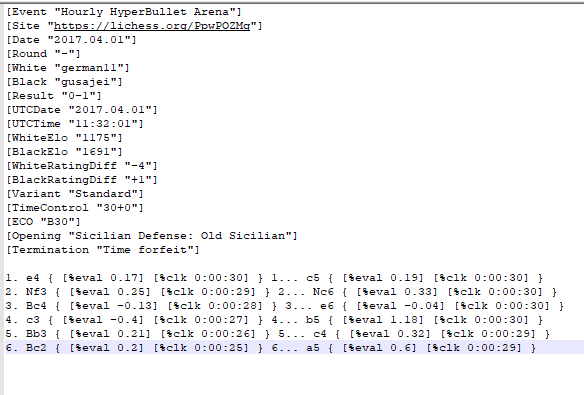
\includegraphics[scale=0.5]{PGN_data.PNG}
    \caption{Sample PGN Data}
\end{figure}

As can be seen in the above sample data, we get the set of moves for every ply along with the strength of the move represented by eval(more on that later),and metadata for the game and players involved.  

\section{Exploratory Data Analysis and Pre-processing}
\begin{figure}[h]
\centering
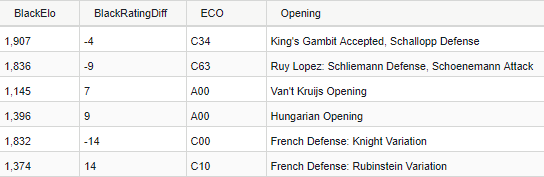
\includegraphics[width=0.5\textwidth]{Dataset.PNG}
\caption{Lichess Data imported as CSV}
\end{figure}
\subsection{Important Attributes}
Most of the data obtained from Lichess is self-explanatory but it would be useful to elaborate some important attributes that have been used for the analysis of this work.
\begin{enumerate}[(i)]
    \item \textbf{Event:} The variant of game in question. After the above pre-processing, 4 variants remained in our dataset, viz. Blitz/Bullet/Classical/Correspondence. As mentioned earlier, we did merge similar variants played under different different event types into one variant.
    \item \textbf{ECO (Encyclopedia of Chess Openings)}\cite{ECO}: A 3 character code which indicates the kind of opening sequence of moves in the game. The format is $<$alphabet$>$ followed by 2$<$numerals$>$. The alphabet indicates the type of opening sequence and the numerals represent the sub-type. This can be considered a more structured and precise way of representing the opening move in comparison to the free text way of specifying an opening. eg. The ECO classifies the 'English Opening' under A10 to A39.
    \item \textbf{Termination:} The different ways in which the game can end viz. Terminated/Normal/Unterminated/Rule Infraction/Death/Emergency/Time forfeit.
    \item \textbf{Numeric Annotation Glyph \cite{NAG}:} We also retrieve the comments or NAGs from the PGN file. Unfortunately, for the dataset we picked from Lichess we only came across 3 distinct values of NAGs in the all the games we did parse, a poor move, a questionable move or a blunder. The notation does allow for positive moves like good, very good and interesting move too. We allot scores, albeit negative scores based on how many of these poor moves were made. These are allotted after the game retrospectively.
    \item \textbf{Center/Diagonal Squares Controls:} We also gather information of how many pieces of White and Black are attacking the central squares E4, E5, D4 and D5. Based on some analysis and readings we concluded that this generally indicates how well either player is playing as control over center squares is widely regarded as indicator of dominance in the game. This is definitely something players strive for during the opening and during the middle phase of the game. But this is not true during the finishing stages of the game. This can be seen from the visualization in figures 3 and 4. Players with higher ELO generally have slightly higher center control than players with lower ELOs. Also note, that mean center control in the end phase of games is more skewed towards 0 compared to the open and mid phases. Based on this analysis, we too split our centre control scores into 3 separate attributes, one for each phase. 
    
    \begin{figure}[!ht]
      \centering
        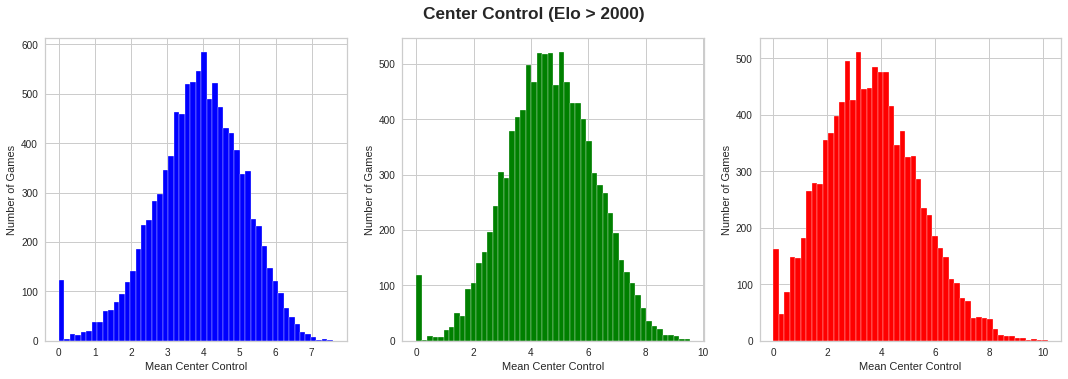
\includegraphics[width=0.5\textwidth]{GT2k_CC.png}
        \caption{Center Control Over Phases For Players with ELO $>$ 2000}
    \end{figure}
    
    \begin{figure}[!ht]
      \centering
        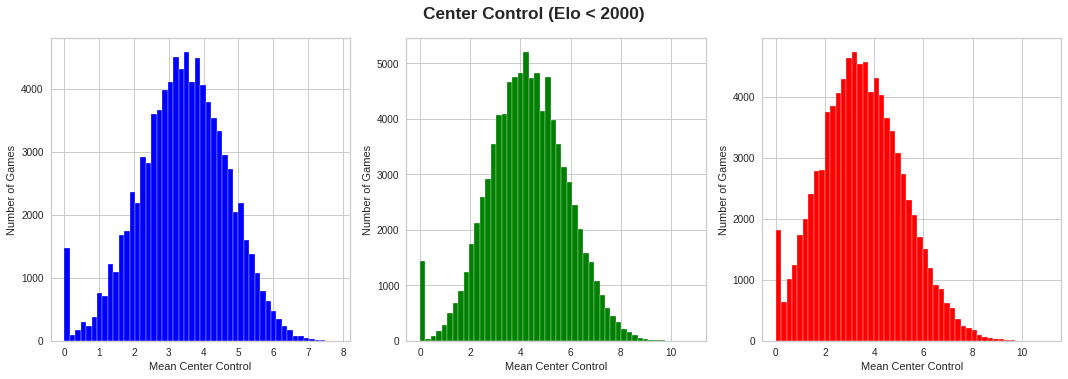
\includegraphics[width=0.5\textwidth]{LT2k_CC.png}
        \caption{Center Control Over Phases For Players with ELO $<$ 2000}
    \end{figure}
\end{enumerate}
\subsection{Preprocessing}
For pre-processing we started out by first imputing the comments column in the CSV itself and thereafter removing some of the unwanted attributes like Site, Date, Black Player, White Player and Round from the created dataframe as they were of no use in determining the player rankings. Also, to maintain the homogeneity in the data, similar event types were merged for better results, eg. 'Rated Blitz Game' and 'Rated Blitz Tournament' were combined as 'Blitz'. Coming to the actual moves sequence, as they are given separately for each ply of moves, we combined them together in a single list to represent the entire state of a game. Additionally, the eval information was provided only for 15\% of the games so we discarded those instead choosing to obtain that data from the source (Chess Engine) itself and for all the moves that we were analysing.

\subsection{Challenges}
\begin{enumerate}[(i)]
    \item \textbf{Familiarity with the PGN format:} Even though we had played chess before, we were not aware the extent to which its used as a potential research tool for looking at problems. We familiarized ourselves with the various Chess openings, game variants, what each specific symbol in a PGN means, how Chess Engines actually work for a given specific depth etc.
    \item \textbf{Handling the volume of data:} Given the huge repository of Chess PGNs available at Lichess with each file running into GBs worth of data, we had to figure out a way to process the files effectively without hitting a roadblock in the first stage itself. To get around this, we built a Python pipeline which would take a PGN file and in addition to parsing the moves and dumping the data to a CSV, also performed some computations on it in conjunction with the Python Chess API to give us the features we needed.
    \item \textbf{Computational Deficiency:} We had a way to convert the source data, our PGN files, into a format that we could easily analyse, CSV files with extracted information. But we struggled to convert the PGNs to CSVs as it the conversion took hours to achieve. As a rough figure, it would take us 12-15 hrs to parse through 50k games on our personal laptops as well as Google Colab. Given that these computations had nothing to do with matrices or tensor calculations, having the extra GPU power did not help. In order to overcome this challenge, we used the Seawulf cluster and split our workload over 13 different nodes. Each node was responsible for converting data for 10k games. The added computational power and ability to process the data on several nodes in parallel effectively reduced the lead time. Finally, we were able to extract data for close to 125k games in close to 2 hours.
    \item \textbf{Choice of Model:}
    In the initial stages while building our baseline model, we were in two minds whether to approach the problem as a classification or discrete value prediction (Regression). The classification approach would make our life a bit easier with ranges of ranks to predict but we figured that with real in-depth analysis the regression models should display good results as well. In the end we decided to use a hybrid approach and create two different models just to ensure that our regression results complement the ones we obtain from classification as well. 
\end{enumerate}

\section{Feature Engineering}
Since the moves cannot be directly fed into machine learning models, most of our efforts in this project were spent on intelligent feature engineering to quantify the moves and infer as much information as we can about the strategy of the players from them.

First of all, our main goal was prediction of Elo rankings based on the player moves, hence we divided the half moves between White and Black.This meant that rather than treat the games as a single entity, we created two rows for each game, one for Black and another for White with the corresponding features created from their half moves and their corresponding Elo Rankings as the labels.

Based on our knowledge of the game, online sources and the 5-year old Kaggle challenge \cite{KaggleFindingElo}, we created 58 features, which can be broadly categorized as 'Move Count' based, 'Board Control' based and 'Statistics based', some of which are explained below:

\begin{figure*}
	    \centering
		\begin{subfigure}{0.3\textwidth}
			\centering
			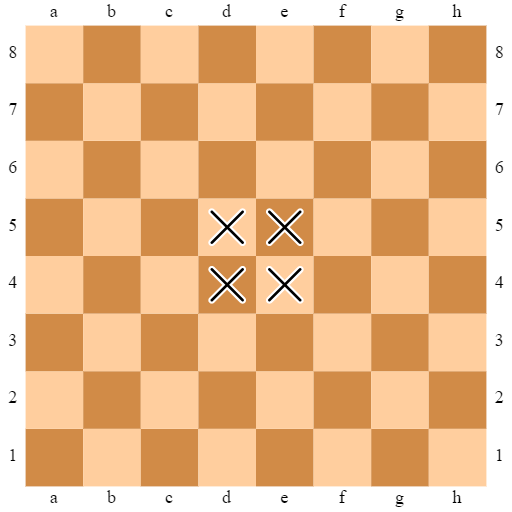
\includegraphics[width=4cm,height=4cm,keepaspectratio]{center-control.png}
			\caption{Center Control Squares}
			\label{fig:center-control}
		\end{subfigure}
		\begin{subfigure}{0.3\textwidth}
			\centering
			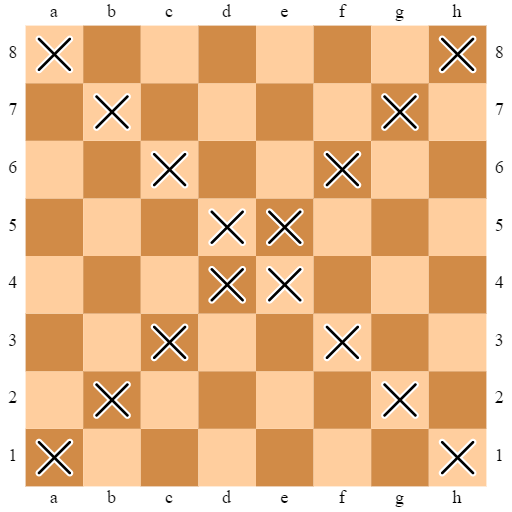
\includegraphics[width=4cm,height=4cm,keepaspectratio]{diagonal-control.png}
			\caption{Diagonal Control Squares}
			\label{fig:diagonal-control}
		\end{subfigure}
		\begin{subfigure}{0.3\textwidth}
			\centering
			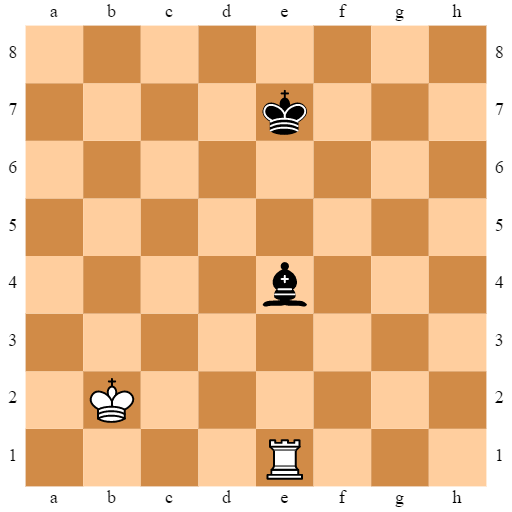
\includegraphics[width=4cm,height=4cm,keepaspectratio]{pinned-piece-example.png}
			\caption{Pinned Piece - Black Bishop}
			\label{fig:pinned-pieces}
		\end{subfigure}
		\caption{Board Control Based Feature Representation}
	\end{figure*}

\begin{enumerate}[I]
    \item \textbf{Moves Count Based:}
\begin{enumerate}[(i)]
    \item \textbf{Opening Move:} Based on whether the Opening Sequence was a 'Defence' or 'Attack/Reversed Defence', the categorical column was set to 1 for Black or White respectively.
    \item \textbf{(Player/Opponent)Captures:} The number of pieces captured by a player and the number of pieces lost. Captures by the opponent are represented with a negative value to punish the player.
    \item \textbf{Checks/Check Mates:} The number of times player forces a 'check' on the opponent or finishes them off with a mate.
    \item \textbf{Moves made by Significant Pieces:} The number of times significant pieces, Queen(Q), King(K), Knight(N), Bishop(B) and Rook(R) move. We also capture the first time these pieces were moved. (We did NOT mark the first move for each of the Bishops/Knights/Rook individually for the first move.)
    \begin{figure}[!ht]
      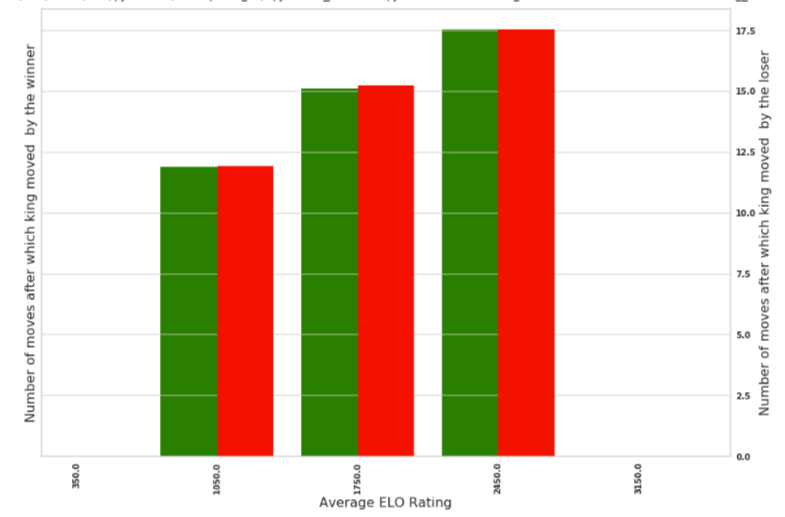
\includegraphics[width=0.5\textwidth]{QueenMovNum.png}
      \caption{Num of moves for Queen vs Elo}
      \label{fig:Queen}
        
    \end{figure}
    
    Our choice of this too was based on some preliminary analysis. In figures \ref{fig:Queen} and 6 we plot number of times Queen and King moved against the Elo rating of the player.\\
    \begin{figure}[!ht]
        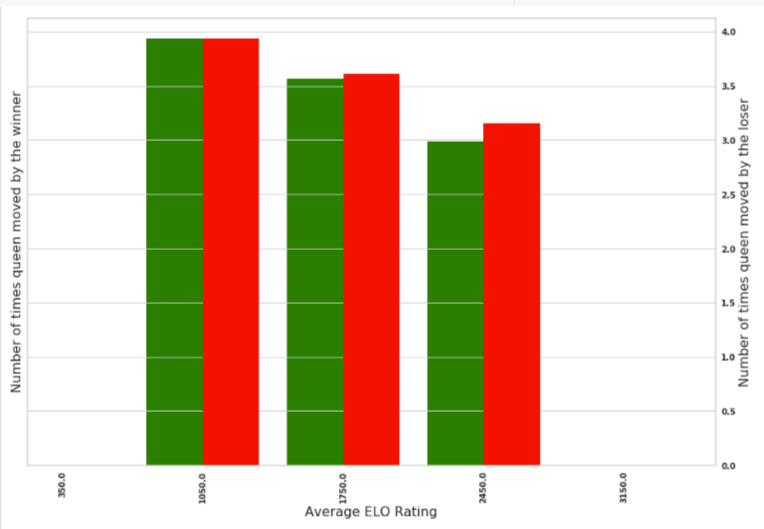
\includegraphics[width=0.5\textwidth]{KingMoveNum.png}
        \caption{Num of moves for King vs Elo}
        \label{fig:King}
    \end{figure}
    
    While players with higher Elo generally move the King more than players with lower Elo, it is the opposite when it comes to the Queen. Similar can also be said about the Bishop, Knight and Root, though the effect is not as prominent as that of the Queen and the King.
    
    
    \item \textbf{Questionable Moves:} Referencing the 'Comments' column from the previous section, some of the moves are annotated with a score from 2/4/6 which indicate a Poor Move/Blunder/Questionable Move respectively. We count the number of instances such a move was played by the player as well as the opponent.
    
\end{enumerate}

    \item \textbf{Board Control Based:}
    \begin{enumerate}[(i)]
        \item \textbf{Special Moves:} Castling(Both Queen side and King side) and which are represented as 'O-O-O/O-O'.
        \item \textbf{Promotion:} Promotion of pawn to special pieces represented by '=X' where X is the piece to which the pawn transforms too.
        \item \textbf{Board Center Control:} These are some of the most important calculated and derived features that we have used. If the game has more than 10 moves, we divide the game into three phases-Open, Mid and End moves. We define the Open-Phase as the first 10 moves, the Mid-Phase to be moves 11 to 28 and move 29 on wards is the End Phase. 10 moves is generally regarded as the number of moves used to define the opening phase. We chose 28 for end of the Mid-phase based on the average move number when the King is first moved in the game. Then, by the use of python-chess, we calculate the count of attackers on the center squares (4 middle squares) which are considered the most important as far as controlling the board space area is concerned.
        \item \textbf{Board Diagonals Control:} Similar to Center Control, we also define the Diagonal Control based on the number of pieces that are attacking the diagonal squares. Also, we split the Diagonal Control metrics into 3 phases like as discussed above.
        \item \textbf{Number of Pinned Pieces:} This feature captures the number of pieces that are pinned to the King. These pieces cannot move without putting the King under a check and hence are 'pinned' to their square. It is an indicator of how many choices a player has at any stage. Having more pieces pinned is generally an indicator where the player might get locked down and that of a poor Elo rating.

    \end{enumerate}
        
    \item \textbf{Statistics Based:}
    \begin{enumerate} [(i)]
        \item \textbf{StockFish Analysis:}As mentioned earlier, we discarded any eval information provided with the PGN as eval was marked only for a few games and we wanted it for as many games as possible to make useful predictions. The official term for eval is ACPL (Average Centi Pawn Loss per move) which is an indicator how good or bad a move was in measures of Centi Pawn units which is generally considered a value of 1/100. We obtained the corresponding values for about 100k games and used them as features for our analysis.
        
        \item \textbf{Mean Player/Opponent Gain:} 
        From the evals that we obtained above, we can calculate the Gain or Loss per move for a player by measure the change in evals between plys. We calculated the mean of the Gain thus obtained which proved to be a good addition for our model.
        
        \item \textbf{Difference Prediction between Elo Ratings of Players:} Based upon our various readings throughout the Project phase, we came across \cite{PredicteDiffBetweenElo} where an algorithm was designed to predict the Elo rating difference for 2 players based on a single/set of games. The essence of the algorithm is still in eval but rather than depend only the eval, a series of evals are used to create a probability distribution which is in turn used to calculate a parameter 'D' which  is the \textbf{perceived} difference between the ratings of two players. The distribution of perceived Elo difference over all games can be seen in \ref{fig:PerceivedInDiff}. Notice, that number of games for which predicted Elo differences small are less is high. This is inline with what we expect - players with similar ratings are more like to play against each other.
        
        \begin{figure}[!ht]
            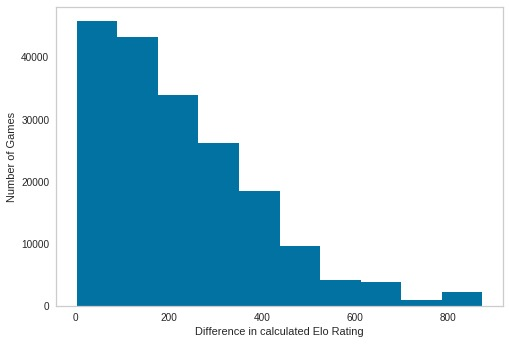
\includegraphics[width=0.5\textwidth]{diff.jpeg}
            \caption{Distribution of Perceived Elo Rating Difference}
            \label{fig:PerceivedInDiff}
        \end{figure}
    
    \end{enumerate}
\end{enumerate}

Finally, we end up using the features as seen in \ref{fig:TrainingColumns}. As per feedback from our Mid-Project Report we can see the correlation matrix in \ref{fig:Correlation} as requested.

\begin{figure}
	\centering
	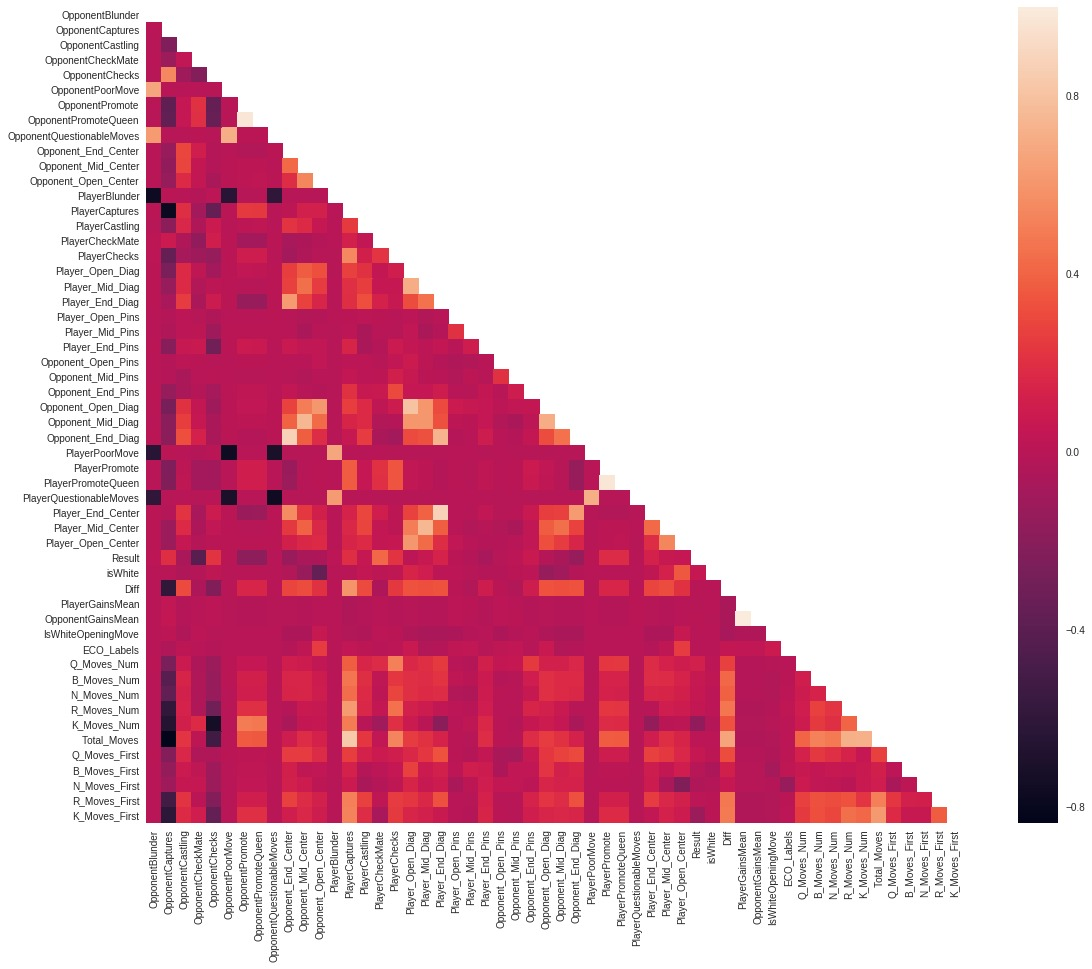
\includegraphics[width=4cm,height=4cm]{correlation.jpeg}
	\caption{Correlation Matrix of Features Used}
    \label{fig:Correlation}
\end{figure}
	
\begin{figure}
	\centering
	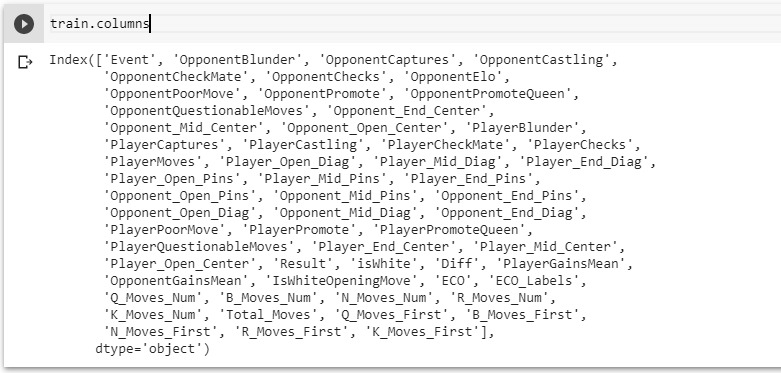
\includegraphics[width=4cm,height=4cm,keepaspectratio]{Columns.jpeg}
    \caption{Training Features}
    \label{fig:TrainingColumns}
\end{figure}
        
\section{Methods}
\subsection{Baseline:}
    Given the nature of the problem at hand, the most natural approach is to try a regression model to fit the features that we created as described earlier. We tried a Linear regression model based on the basic features that could be directly obtained from the moves sequence to have a good baseline models to build upon. \\The combination of 13 features considered for the baseline model were:
\begin{enumerate} [(a)]
    \item Result
    \item isWhite
    \item TotalMoves
    \item Number of Checks/Mates
    \item Poor/Questionable/Blunder Moves of Player/Opponent (From Commentary)
\end{enumerate}
The results obtained from our baseline model as outlined in the Results section helped us gain confidence enough that starting out with regression was the right approach and we could go from 13 basic features to a 58 features rich model which gave us considerable improvements over the baseline.
\subsection{Intermediate and Final:}\\
After finalizing our approach we set to work to improve our baseline model in an incremental fashion. By the time we reached the mid-project report stage we had 39 hand crafted features with the statistical features being saved for the final iteration. Finally, with all the features worked out we applied them to regression models of varied complexity starting from Linear to Random Forest Regressor and XG Boost Regressor. 

\section{Extended Work - Deep Learning:}
\begin{figure}[!ht]
    \centering
    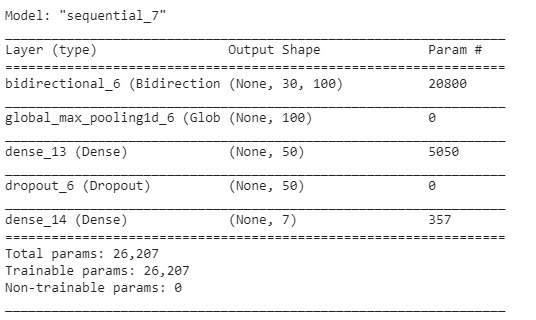
\includegraphics[scale=0.45]{LSTM_Architecture.jpeg}
    \caption{Bi-LSTM Model Architecture }
    \label{fig:LSTM}
\end{figure}
As mentioned in the future work of our previous iteration from mid-sem project report, we tried to pursue the ambitious goal of applying deep learning models to the move sequence to replicate a sort of time-series analyses. The architecture consisted of a state of the art Bidrectional LSTM layer with  MaxPooling concatenation and finally a Dense layer with 'softmax' activation for classification. The sequence of gains was limited at 30 after data analysis and for players with lesser moves the gains sequence was padded and for those with greater number of moves truncated. For our purpose, we used the sequence of gains scored by players in their games to predict :
\subsection{Classification of Elo Ratings:}
Given our regression results we divided the player ranking in our dataset into four ranges:
\begin{enumerate}
    \item $<1000$
    \item $1000-1500$
    \item $1500-2000$
    \item $>2000$
\end{enumerate}
With a 500 ranks range we suspected we would get decent enough accuracy for predicting classes. Sure enough, as described in the Results section we obtained over 60\% accuracy with the dominating classes showing the best accuracy.\\


\subsection{Classification of Game Variant:}
With a Dense layer classification model architecture in place, we extended our scope to include a basic prediction model for Game Type or 'Events' in the dataset. As mentioned in the Pre-processing section, we combined all the games into the following four classes:
\begin{enumerate}
    \item $Blitz$
    \item $Bullet$
    \item $Classic$
    \item $Correspondence$
\end{enumerate}
Since using the Clock information provided in the PGN would directly correlate to the game variant and we were only interested in the move sequence analysis, we applied the same approach as in Elo Rankings classification to treat this is a Time-Series based prediction task. Again, since most of the entries in the dataset were for Blitz and Bullets the results as in the next section reflected that. Even after applying random resampling and upsampling of the minority classes we couldn't see any improvements in the results. Maybe this should be something that needs further investigation.

\section{Results}

\subsection{Regression over Elo Ratings}
As part of our experiments the models were initially run on a smaller dataset of 20000 games. Given that we split the predictions to be separate, we made predictions with a Mean Absolute Error(MAE) of around 155 for Linear Regression and 150 for Random Forest Regressor. We then pumped more data in, in hopes of improving the MAE but only managed a small bump. Feeding the model with 10 times the initial number of games, the MAE was closer to 147.37. We also performed predictions using XGBoostRegressor which gave us an MAE of 148.83. The results are displayed in table \ref{tab:baseline-results} and \ref{tab:final-results} for baseline and final results for our main task.

\begin{table}[]
\begin{tabular}{|l|l|l|l|}
\hline
 & LR & RFR & XGBR \\ \hline
RMSE & 205.08 & 204.61 & 204.45 \\ \hline
MAE & 163.44 & 163.24 & 163.08 \\ \hline
\end{tabular}
\caption{Baseline Results (LR: LinearRegressor, RFR: RandomForestRegressor, XGBR: XGBoostRegressor)}
\label{tab:baseline-results}
\end{table}

\begin{table}[]
\begin{tabular}{|l|l|l|l|}
\hline
 & LR & RFR & XGBR \\ \hline
RMSE & 192.12 & 185.81 & 187.56 \\ \hline
MAE & 152.74 & 147.37 & 148.83 \\ \hline
\end{tabular}
\caption{Final Results (LR: LinearRegressor, RFR: RandomForestRegressor, XGBR: XGBoostRegressor)}
\label{tab:final-results}
\end{table}

\subsection{Range of Elo}
Given that we were getting of RMSE of LR, we wanted to try classification-based approach by trying to classify the in the ranges of ELO. We get an accuracy of 64\% by analyzing the games based on time-series data. The results can be seen in \ref{tab:elo-range-classification-results}. The models created are vanilla model with little complexity giving an excellent accuracy of 64\%. Further enhancements can be made in this direction to improve the accuracy from 64\%.

\begin{table}[]
\begin{tabular}{|l|l|l|l|l|}
\hline
Elo Range & Precision & Recall & F1 & Support \\ \hline
1000-1500 & 0.55 & 0.21 & 0.3 & 21319 \\ \hline
1500-2000 & 0.65 & 0.91 & 0.76 & 38488 \\ \hline
\textless{}1000 & 0 & 0 & 0 & 135 \\ \hline
\textgreater{}2000 & 0 & 0 & 0 & 1906 \\ \hline \hline
Accuracy &  &  & 0.64 & 61848 \\ \hline
Macro Avg & 0.30 & 0.28 & 0.27 & 61848 \\ \hline
Weighted avg & 0.59 & 0.64 & 0.58 & 61848 \\ \hline
\end{tabular}
\caption{Elo Range Classification Results}
\label{tab:elo-range-classification-results}
\end{table}


\subsection{Game Type Classification}
We tried to classify the games based on the game type. We purposely kept out the time field since there is a direct correlation between type Blitz and the time of the game. Results can be seen in \ref{tab:classification-results}

\begin{table}[]
\begin{tabular}{|l|l|l|l|l|}
\hline
Game Type & Precision & Recall & F1 & Support \\ \hline
Blitz & 0.34 & 0.97 & 0.5 & 21319 \\ \hline
Bullet & 0.77 & 0 & 0 & 38488 \\ \hline
Classic & 0.01 & 0.04 & 0.01 & 135 \\ \hline
Corres. & 0 & 0 & 0 & 1906 \\ \hline \hline
Accuracy &  &  & 0.34 & 61848 \\ \hline
\begin{tabular}[c]{@{}l@{}}Macro Avg\end{tabular} & 0.28 & 0.25 & 0.13 & 61848 \\ \hline
\begin{tabular}[c]{@{}l@{}}Weighted Avg\end{tabular} & 0.59 & 0.34 & 0.18 & 61848 \\ \hline
\end{tabular}
\caption{Game Type Classification Results}
\label{tab:classification-results}
\end{table}

\section{Conclusion}
Starting with working knowledge of chess, this was an enlightening experience. Our main task was the prediction of Elo rankings of players based on their moves in chess games obtained from Lichess.com. From a baseline model with RMSE of 205 we were able to bring the prediction within a confidence of RMSE of 187 through smart feature engineering and use of available chess engine APIs. Further, we were also able to apply a deep learning model to the task of classifying Elo ratings and also the Game variant with baseline level accuracy. Those prove to some degree that various aspects of chess move sequences can be modelled as Time Series analysis to obtain appreciable results.

\bibliography{naaclhlt2019}
\bibliographystyle{acl_natbib}

\end{document}
